\documentclass[10pt,twocolumn]{article}

\usepackage{titlesec}

\titleformat{\section}{\normalfont\Large\bfseries}{\thesection}{2em}{}
\titlespacing*{\section}{1pt}{*1}{*1}

% Page layout
\usepackage[a4paper,margin=1in]{geometry}

% Font settings (choose any font package you prefer)
\usepackage{mathptmx}  % Times New Roman font
\usepackage{fontspec}

% Hyperlinks
\usepackage{hyperref}

% Colors
\usepackage{xcolor}

% Tables
\usepackage{booktabs}

% Figures
\usepackage{graphicx}
\usepackage{afterpage}


% Title and Author information
\title{\vspace{-2cm}Global Attention Is All Mutagenic Molecules Need}
\author{Ludek Cizinsky (ludek.cizinsky@epfl.ch)}
\date{\today}

\begin{document}
\maketitle

\section{Introduction}
This report investigates the use of Graph Neural Networks
for mutagenicity prediction of chemical compounds. 
The mutagenicity of a chemical compound is a binary property
indicating whether the compound is likely to cause mutations
in living organisms. The prediction of mutagenicity is an
important task in drug discovery, as mutagenic compounds
are likely to be carcinogenic. The dataset used for this task is the 
\textit{MUTAG} dataset \cite{mutag}, which contains 188 chemical compounds.
The report first focuses on building optimal Graph Neural Network using
only node features. Then, the report investigates the use of edge features
as a way to improve the performance of the model. All experiments are
with associated code are available at \href{https://github.com/ludekcizinsky/epfl-cs502/tree/main/coursework/homeworks/hw2}{\textcolor{blue}{Github}}. 

\section{Dataset}\label{sec:dataset}
The \textit{MUTAG} dataset \cite{mutag} contains 188 chemical compounds with
binary labels indicating whether the compound is mutagenic or not. In total,
there is 63 mutagenic and 125 non-mutagenic compounds. Each compound is represented
as a graph. Each node and edge has is associated with one hot encoded feature vector
indicating type of the node (atom) and type of the edge (bond). It is important to note
that the labels are unvevenly distributed, with two thirds of the compounds being mutagenic.
The skew in the labels is favorable for the downstream task, however, the trained
models might be as a result more biased towards predicting mutagenic compounds.


The feature vectors were mapped to double precision floating point numbers to
increase the numerical stability of the model. In addition, based on the provided
edges indices, the adjacency matrix was constructed.


% TODO: maybe define what is overall the goal --> build nice features
% TODO: add figure showing the whole pipeline
% TODO: add the explanation of global softmaxing
\section{Methodology}\label{sec:methodology}
On a high level, GNN's goal is to transform the given
graph into a vector representation, which can then be used
for the downstream task, in this case binary classification.

The first part of the experiment focuses on building a GNN purely
based on transformation of the initial node features. The experiment compares the performance of the
three types of convolutional layers: Normal Graph Convolution (\texttt{NormConv}), 
GraphSAGE (\texttt{SAGEConv}) and Graph Attention (\texttt{GATConv}).

\texttt{GCNConv} first computes representation of each node by aggregating
over the features of its neighbors. Then, the representation is transformed
using a linear layer, and linearly transformed representation of the node is added.
The \texttt{SAGEConv} extends the \texttt{GCNConv} by allowing the user to 
choose the aggregation function, i.e., one can for instance use \texttt{max pooling}
strategy to obtain the aggregate instead of mean. Finally, the \texttt{GATConv} aggregates
the neighbors using attention weights, which indicate the importance of each neighbor 
for the representation of the node. The attention weights are learned during training.

In the second part of the experiment, the edge features are used to improve the performance
of the model. In general, every node convolution layer is now followed by en edge convolution.
This way the model can learn to incorporate the edge features into the node representation.
Two types of edge convolutions are used: Graph Edge Sum \texttt{ESUMConv} and Graph Edge Attention
(\texttt{EATTConv}).

The idea behind \texttt{ESUMConv} is that each node's representation should be updated 
by sum of the edge features that are associated with the given node. Thus, the node's
representation no longer depends on the type of its neighbors, but also on the type of
connections with its neighbors. The \texttt{EATTConv} extends the \texttt{ESUMConv}
idea by using attention weights to indicate the importance of each edge feature. Importantly,
in contrast to the \texttt{ESUMConv}, can be set to not only aggregate over the node's associated edges,
but also over over all ages in the graph. In the remaining of the report, the \texttt{EATTConvL} will refer
to the local version while \texttt{EATTConvG} will refer to the global version.

Finally, after the pass through the given number of convolutional layers, the transformed
node features are reduced via one of the two pooling layers, \texttt{MaxPool} or \texttt{MeanPool}, 
into a one dimensional embedding representing the whole graph. This is then fed through
a linear layer to obtain the final prediction. Given the model's output, the binary cross entropy
loss is used to compute the loss, which is then used to update the model's parameters.

\begin{figure*}
    \centering
    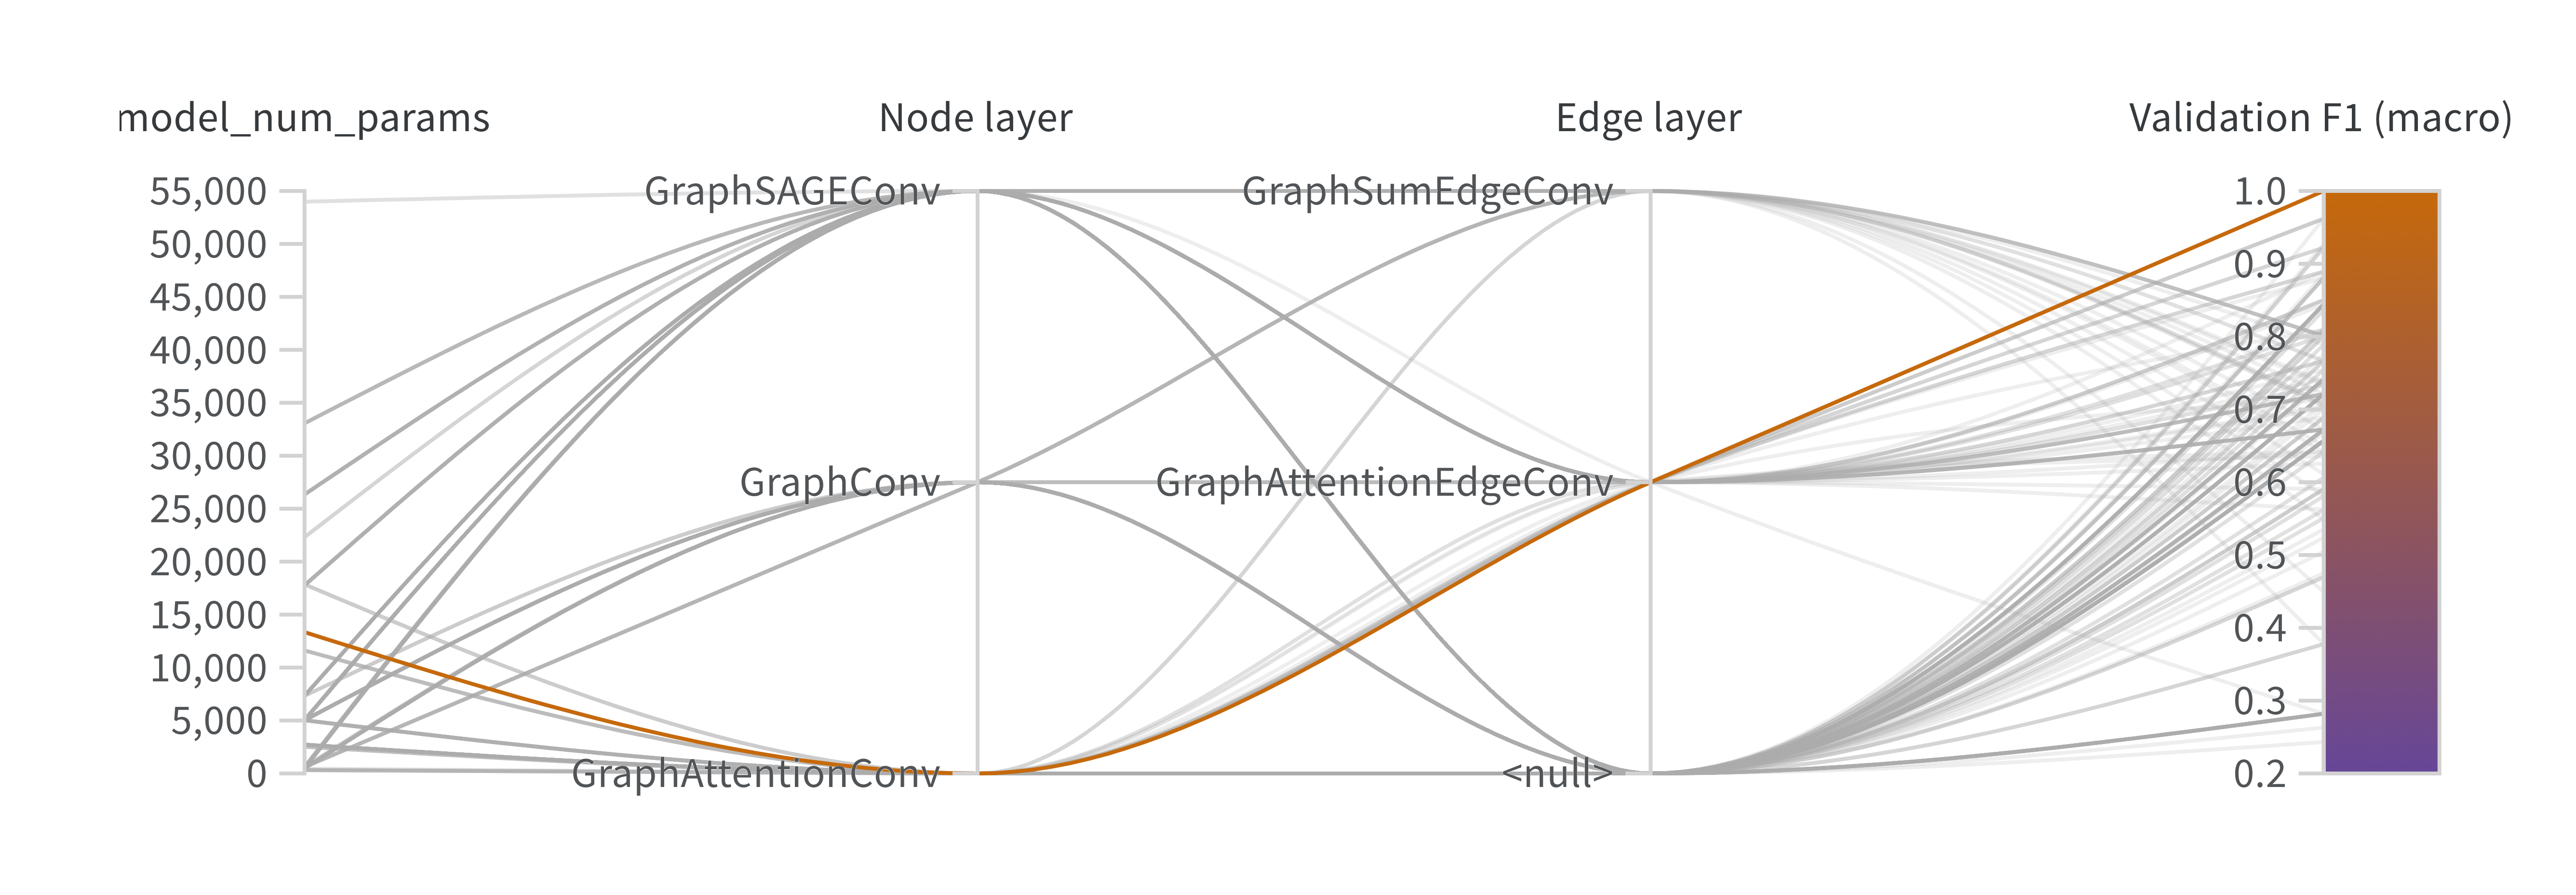
\includegraphics[width=1\textwidth]{figures/hyperparams.png}
    \caption{Relationship between model complexity, type of node and edge convolution and the model's performance. The highlighted line indicates the best performing model.}
    \label{fig:hyperparams}
\end{figure*}

Last but not the least, macro averaged F1 score is used as the metric to evaluate the performance
of all models. This means that we take into account model's ability to correctly classify both
mutagenic and non-mutagenic compounds. % Importantly, the F1 score takes into account both precision and 
% recall and as such can be relied on even in the case of unbalanced labels.

\section{Experiments}
\begin{table}[!ht]
    \centering
    \begin{tabular}{llccc}
    \toprule
    \textbf{Layer} & \textbf{Depth} & \textbf{Val Loss} & \textbf{F1-Macro} \\
    \midrule
    \texttt{Norm} & M & 0.41 & 0.74 \\
    w/\texttt{EATTG} & L & 0.32 & 0.85 \\
    \midrule
    \texttt{SAGE} & L & 0.26 & 0.88 \\
    w/\texttt{EATTG} & L & 0.17 & 0.89 \\
    \midrule
    \texttt{GATT} & L & 0.33 & 0.96 \\
    \textbf{w/\texttt{EATTG}} & \textbf{L} & \textbf{0.19} & \textbf{1.00} \\
    \bottomrule
    \end{tabular}
    \caption{Experiment Results. Depth of the model is indicated by Medium (M, 2 layers) and Large (L, at least 3 layers).}
    \label{tab:results}
\end{table}

The table \ref{tab:results} summarizes the results of the experiments. Each section
corresponds to one particular type of convolutional layer applied on nodes. The second
row then indicates the performance of the model when the edge features are integrated using
the better performing method. We can clearly see that as the node convolutional layers
are getting more sophisticated, the model's performance is improving. Further, it is important to notice
that majority of the models consisted of at least three convolutional layers (L). This indicates
that the model needs to be sufficiently complex to be able to learn the task. 

Finally, as the title of this report suggests, enhancing the node convolutional layers with
the aggregated edge features via \texttt{EATTG} improves the performance accross all models.
This is especially true for the \texttt{Norm} model, where the performance
improves by 11\%. The other two models, on the other hand, already
performed very well without the edge features, and thus the improvement is only marginal, yet
still significant. 

TODO: add test evaluation performance

\section{Discussion}

\begin{figure}[!ht]
    \centering
    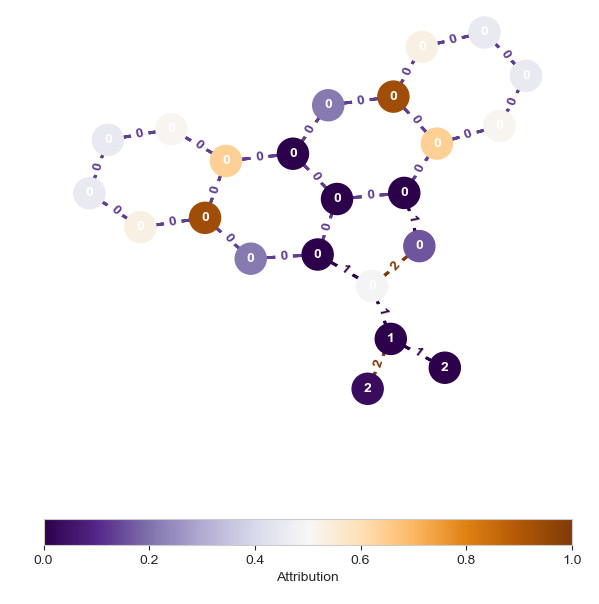
\includegraphics[width=0.35\textwidth]{figures/interpret.png}
    \caption{Visualization of the relative nodes' and edges' importance for the prediction of the graph's label.}
    \label{fig:attribution}
\end{figure}

The results clearly suggest that the attention mechanism is the best method for aggregating
both node and edge features. This is not surprising, as the attention mechanism proved to be working
well in many other domains \cite{transfomers}. However, the most important finding is that for the specific task of
mutagenicity prediction, consideration of all nodes / edges, i.e., the global approach is superior
to the local approach. Figure \ref{fig:attribution} tries to explain why this is the case. It shows the
relative importance of each node and edge for the prediction of the graph's label. The importance is
computed using Integrated Gradients approach \cite{attribution}. It is clear that the final prediction is
based only on a small subset of nodes and edges (orange/brown colour) which do not need to be neccessary 
connected. Last but not the least, Figure \ref{fig:hyperparams} shows the path towards the best performing models. Despite 
the small number of parameters, attention based model's are able to outperform other more complex models. 
%The importance of using the global approach is further supported by the lower performance of those models' using \texttt{ESUM} for 
% edge aggregation, which is a local approach, i.e., only the edges associated with the given node are considered.

\section{Conclusion}
To conclude, this report investigated the use of Graph Neural Networks for the task of mutagenicity prediction. 
The results show that both node and edge features are important for the task. Further, the global attention mechanism
proved to be the best method for aggregating both node and edge features. Future work could focus on
testing the proposed model on other datasets and tasks.

\newpage
\bibliographystyle{abbrv}
\bibliography{references}

\end{document}